\documentclass[1p]{elsarticle_modified}
%\bibliographystyle{elsarticle-num}

%\usepackage[colorlinks]{hyperref}
%\usepackage{abbrmath_seonhwa} %\Abb, \Ascr, \Acal ,\Abf, \Afrak
\usepackage{amsfonts}
\usepackage{amssymb}
\usepackage{amsmath}
\usepackage{amsthm}
\usepackage{scalefnt}
\usepackage{amsbsy}
\usepackage{kotex}
\usepackage{caption}
\usepackage{subfig}
\usepackage{color}
\usepackage{graphicx}
\usepackage{xcolor} %% white, black, red, green, blue, cyan, magenta, yellow
\usepackage{float}
\usepackage{setspace}
\usepackage{hyperref}

\usepackage{tikz}
\usetikzlibrary{arrows}

\usepackage{multirow}
\usepackage{array} % fixed length table
\usepackage{hhline}

%%%%%%%%%%%%%%%%%%%%%
\makeatletter
\renewcommand*\env@matrix[1][\arraystretch]{%
	\edef\arraystretch{#1}%
	\hskip -\arraycolsep
	\let\@ifnextchar\new@ifnextchar
	\array{*\c@MaxMatrixCols c}}
\makeatother %https://tex.stackexchange.com/questions/14071/how-can-i-increase-the-line-spacing-in-a-matrix
%%%%%%%%%%%%%%%

\usepackage[normalem]{ulem}

\newcommand{\msout}[1]{\ifmmode\text{\sout{\ensuremath{#1}}}\else\sout{#1}\fi}
%SOURCE: \msout is \stkout macro in https://tex.stackexchange.com/questions/20609/strikeout-in-math-mode

\newcommand{\cancel}[1]{
	\ifmmode
	{\color{red}\msout{#1}}
	\else
	{\color{red}\sout{#1}}
	\fi
}

\newcommand{\add}[1]{
	{\color{blue}\uwave{#1}}
}

\newcommand{\replace}[2]{
	\ifmmode
	{\color{red}\msout{#1}}{\color{blue}\uwave{#2}}
	\else
	{\color{red}\sout{#1}}{\color{blue}\uwave{#2}}
	\fi
}

\newcommand{\Sol}{\mathcal{S}} %segment
\newcommand{\D}{D} %diagram
\newcommand{\A}{\mathcal{A}} %arc


%%%%%%%%%%%%%%%%%%%%%%%%%%%%%5 test

\def\sl{\operatorname{\textup{SL}}(2,\Cbb)}
\def\psl{\operatorname{\textup{PSL}}(2,\Cbb)}
\def\quan{\mkern 1mu \triangleright \mkern 1mu}

\theoremstyle{definition}
\newtheorem{thm}{Theorem}[section]
\newtheorem{prop}[thm]{Proposition}
\newtheorem{lem}[thm]{Lemma}
\newtheorem{ques}[thm]{Question}
\newtheorem{cor}[thm]{Corollary}
\newtheorem{defn}[thm]{Definition}
\newtheorem{exam}[thm]{Example}
\newtheorem{rmk}[thm]{Remark}
\newtheorem{alg}[thm]{Algorithm}

\newcommand{\I}{\sqrt{-1}}
\begin{document}

%\begin{frontmatter}
%
%\title{Boundary parabolic representations of knots up to 8 crossings}
%
%%% Group authors per affiliation:
%\author{Yunhi Cho} 
%\address{Department of Mathematics, University of Seoul, Seoul, Korea}
%\ead{yhcho@uos.ac.kr}
%
%
%\author{Seonhwa Kim} %\fnref{s_kim}}
%\address{Center for Geometry and Physics, Institute for Basic Science, Pohang, 37673, Korea}
%\ead{ryeona17@ibs.re.kr}
%
%\author{Hyuk Kim}
%\address{Department of Mathematical Sciences, Seoul National University, Seoul 08826, Korea}
%\ead{hyukkim@snu.ac.kr}
%
%\author{Seokbeom Yoon}
%\address{Department of Mathematical Sciences, Seoul National University, Seoul, 08826,  Korea}
%\ead{sbyoon15@snu.ac.kr}
%
%\begin{abstract}
%We find all boundary parabolic representation of knots up to 8 crossings.
%
%\end{abstract}
%\begin{keyword}
%    \MSC[2010] 57M25 
%\end{keyword}
%
%\end{frontmatter}

%\linenumbers
%\tableofcontents
%
\newcommand\colored[1]{\textcolor{white}{\rule[-0.35ex]{0.8em}{1.4ex}}\kern-0.8em\color{red} #1}%
%\newcommand\colored[1]{\textcolor{white}{ #1}\kern-2.17ex	\textcolor{white}{ #1}\kern-1.81ex	\textcolor{white}{ #1}\kern-2.15ex\color{red}#1	}

{\Large $\underline{11n_{30}~(K11n_{30})}$}

\setlength{\tabcolsep}{10pt}
\renewcommand{\arraystretch}{1.6}
\vspace{1cm}\begin{tabular}{m{100pt}>{\centering\arraybackslash}m{274pt}}
\multirow{5}{120pt}{
	\centering
	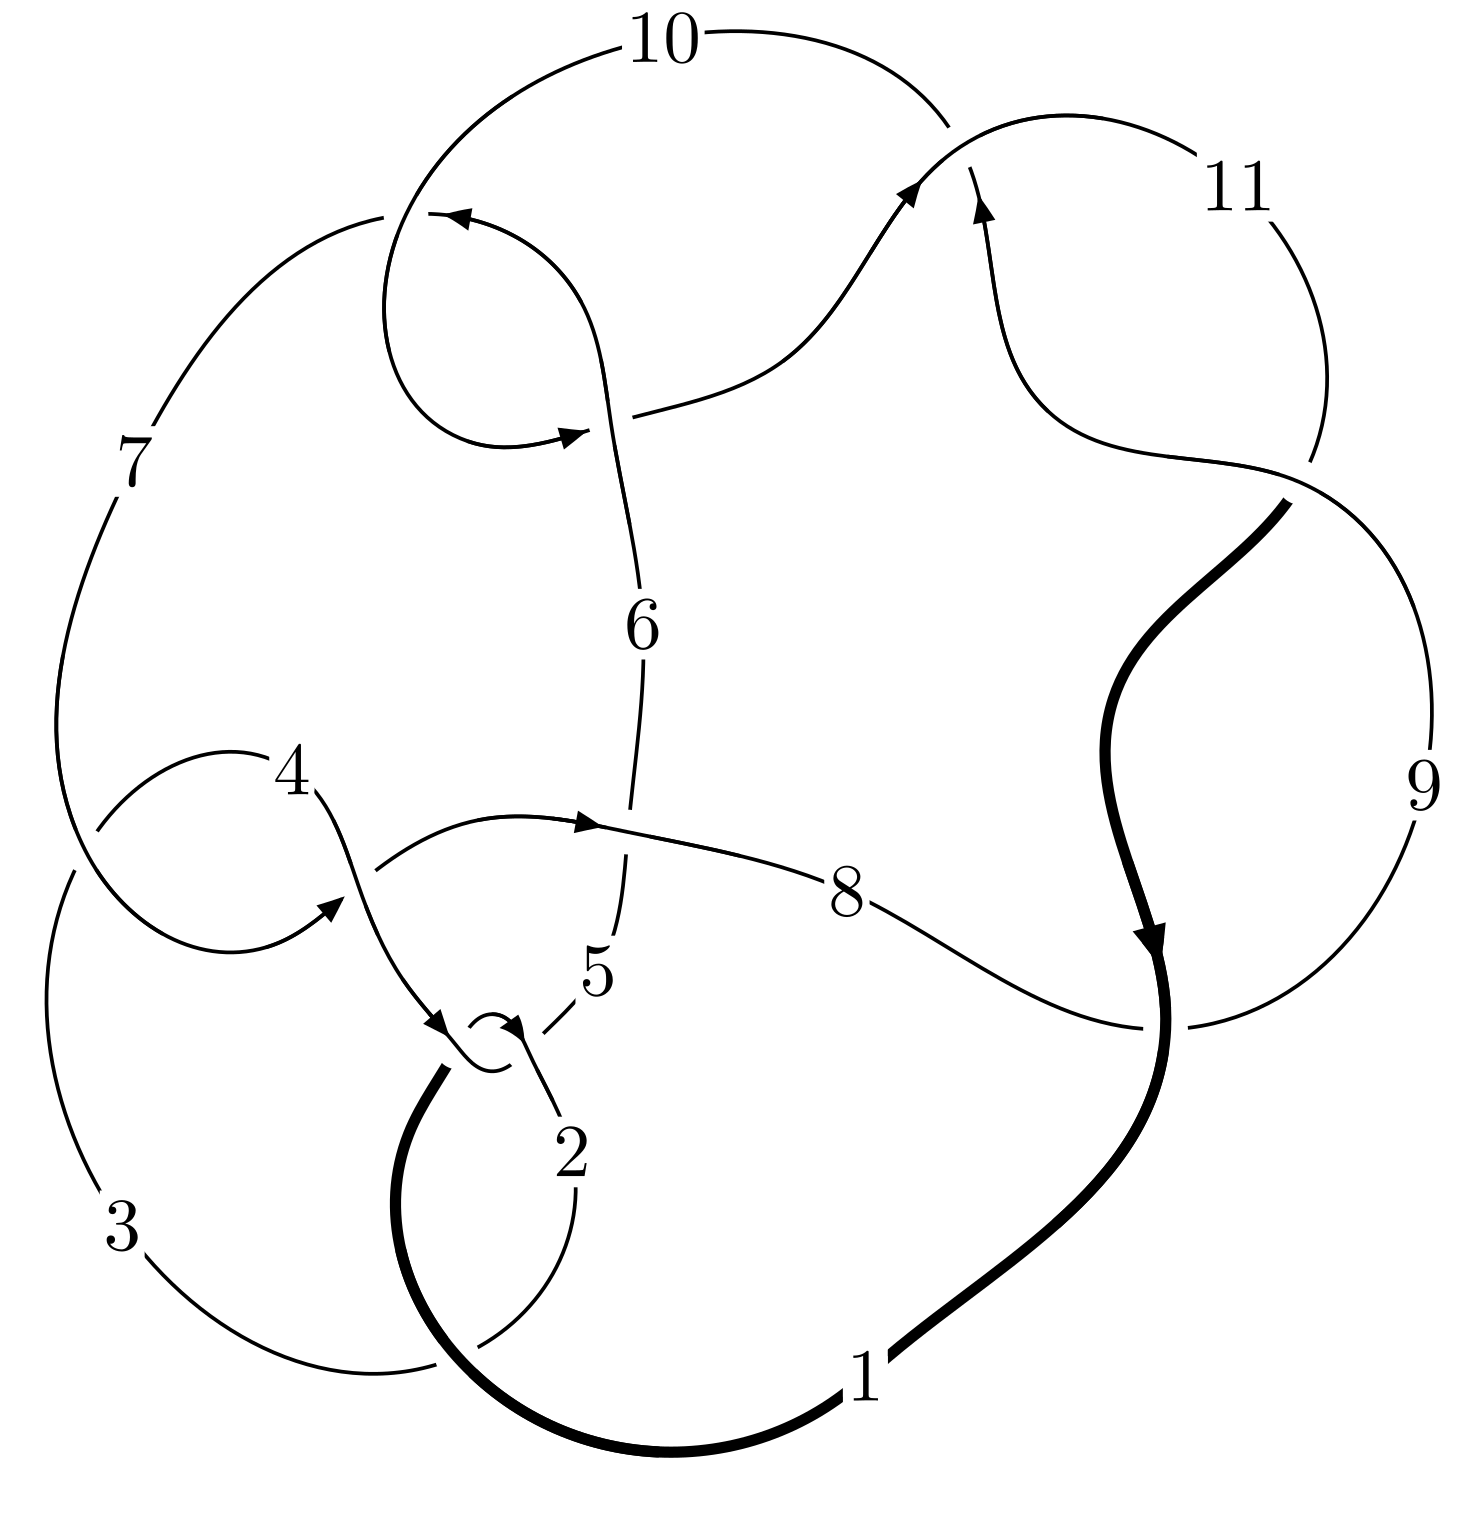
\includegraphics[width=112pt]{../../../GIT/diagram.site/Diagrams/png/646_11n_30.png}\\
\ \ \ A knot diagram\footnotemark}&
\allowdisplaybreaks
\textbf{Linearized knot diagam} \\
\cline{2-2}
 &
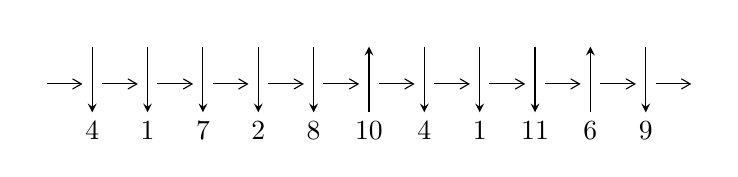
\begin{tikzpicture}[x=20pt, y=17pt]
	% nodes
	\node (C0) at (0, 0) {};
	\node (C1) at (1, 0) {};
	\node (C1U) at (1, +1) {};
	\node (C1D) at (1, -1) {4};

	\node (C2) at (2, 0) {};
	\node (C2U) at (2, +1) {};
	\node (C2D) at (2, -1) {1};

	\node (C3) at (3, 0) {};
	\node (C3U) at (3, +1) {};
	\node (C3D) at (3, -1) {7};

	\node (C4) at (4, 0) {};
	\node (C4U) at (4, +1) {};
	\node (C4D) at (4, -1) {2};

	\node (C5) at (5, 0) {};
	\node (C5U) at (5, +1) {};
	\node (C5D) at (5, -1) {8};

	\node (C6) at (6, 0) {};
	\node (C6U) at (6, +1) {};
	\node (C6D) at (6, -1) {10};

	\node (C7) at (7, 0) {};
	\node (C7U) at (7, +1) {};
	\node (C7D) at (7, -1) {4};

	\node (C8) at (8, 0) {};
	\node (C8U) at (8, +1) {};
	\node (C8D) at (8, -1) {1};

	\node (C9) at (9, 0) {};
	\node (C9U) at (9, +1) {};
	\node (C9D) at (9, -1) {11};

	\node (C10) at (10, 0) {};
	\node (C10U) at (10, +1) {};
	\node (C10D) at (10, -1) {6};

	\node (C11) at (11, 0) {};
	\node (C11U) at (11, +1) {};
	\node (C11D) at (11, -1) {9};
	\node (C12) at (12, 0) {};

	% arrows
	\draw[->,>={angle 60}]
	(C0) edge (C1) (C1) edge (C2) (C2) edge (C3) (C3) edge (C4) (C4) edge (C5) (C5) edge (C6) (C6) edge (C7) (C7) edge (C8) (C8) edge (C9) (C9) edge (C10) (C10) edge (C11) (C11) edge (C12) ;	\draw[->,>=stealth]
	(C1U) edge (C1D) (C2U) edge (C2D) (C3U) edge (C3D) (C4U) edge (C4D) (C5U) edge (C5D) (C6D) edge (C6U) (C7U) edge (C7D) (C8U) edge (C8D) (C9U) edge (C9D) (C10D) edge (C10U) (C11U) edge (C11D) ;
	\end{tikzpicture} \\
\hhline{~~} \\& 
\textbf{Solving Sequence} \\ \cline{2-2} 
 &
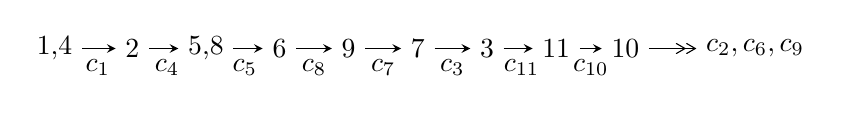
\begin{tikzpicture}[x=25pt, y=7pt]
	% node
	\node (A0) at (-1/8, 0) {1,4};
	\node (A1) at (1, 0) {2};
	\node (A2) at (33/16, 0) {5,8};
	\node (A3) at (25/8, 0) {6};
	\node (A4) at (33/8, 0) {9};
	\node (A5) at (41/8, 0) {7};
	\node (A6) at (49/8, 0) {3};
	\node (A7) at (57/8, 0) {11};
	\node (A8) at (65/8, 0) {10};
	\node (C1) at (1/2, -1) {$c_{1}$};
	\node (C2) at (3/2, -1) {$c_{4}$};
	\node (C3) at (21/8, -1) {$c_{5}$};
	\node (C4) at (29/8, -1) {$c_{8}$};
	\node (C5) at (37/8, -1) {$c_{7}$};
	\node (C6) at (45/8, -1) {$c_{3}$};
	\node (C7) at (53/8, -1) {$c_{11}$};
	\node (C8) at (61/8, -1) {$c_{10}$};
	\node (A9) at (10, 0) {$c_{2},c_{6},c_{9}$};

	% edge
	\draw[->,>=stealth]	
	(A0) edge (A1) (A1) edge (A2) (A2) edge (A3) (A3) edge (A4) (A4) edge (A5) (A5) edge (A6) (A6) edge (A7) (A7) edge (A8) ;
	\draw[->>,>={angle 60}]	
	(A8) edge (A9);
\end{tikzpicture} \\ 

\end{tabular} \\

\footnotetext{
The image of knot diagram is generated by the software ``\textbf{Draw programme}" developed by Andrew Bartholomew(\url{http://www.layer8.co.uk/maths/draw/index.htm\#Running-draw}), where we modified some parts for our purpose(\url{https://github.com/CATsTAILs/LinksPainter}).
}\phantom \\ \newline 
\centering \textbf{Ideals for irreducible components\footnotemark of $X_{\text{par}}$} 
 
\begin{align*}
I^u_{1}&=\langle 
u^{19}-3 u^{18}+\cdots+4 b+8,\;-3 u^{19}-18 u^{18}+\cdots+4 a+9,\;u^{20}+5 u^{19}+\cdots-6 u-1\rangle \\
I^u_{2}&=\langle 
b^4+b^3+3 b^2+2 b+1,\;a,\;u-1\rangle \\
\\
\end{align*}
\raggedright * 2 irreducible components of $\dim_{\mathbb{C}}=0$, with total 24 representations.\\
\footnotetext{All coefficients of polynomials are rational numbers. But the coefficients are sometimes approximated in decimal forms when there is not enough margin.}
\newpage
\renewcommand{\arraystretch}{1}
\centering \section*{I. $I^u_{1}= \langle u^{19}-3 u^{18}+\cdots+4 b+8,\;-3 u^{19}-18 u^{18}+\cdots+4 a+9,\;u^{20}+5 u^{19}+\cdots-6 u-1 \rangle$}
\flushleft \textbf{(i) Arc colorings}\\
\begin{tabular}{m{7pt} m{180pt} m{7pt} m{180pt} }
\flushright $a_{1}=$&$\begin{pmatrix}1\\0\end{pmatrix}$ \\
\flushright $a_{4}=$&$\begin{pmatrix}0\\u\end{pmatrix}$ \\
\flushright $a_{2}=$&$\begin{pmatrix}1\\u^2\end{pmatrix}$ \\
\flushright $a_{5}=$&$\begin{pmatrix}- u\\- u^3+u\end{pmatrix}$ \\
\flushright $a_{8}=$&$\begin{pmatrix}\frac{3}{4} u^{19}+\frac{9}{2} u^{18}+\cdots-\frac{71}{4} u-\frac{9}{4}\\-\frac{1}{4} u^{19}+\frac{3}{4} u^{18}+\cdots-\frac{25}{4} u-2\end{pmatrix}$ \\
\flushright $a_{6}=$&$\begin{pmatrix}-1\\-\frac{1}{8} u^{19}-\frac{1}{2} u^{18}+\cdots+\frac{21}{8} u+\frac{1}{8}\end{pmatrix}$ \\
\flushright $a_{9}=$&$\begin{pmatrix}u^{19}+\frac{15}{4} u^{18}+\cdots-\frac{23}{2} u-\frac{1}{4}\\-\frac{1}{4} u^{19}+\frac{3}{4} u^{18}+\cdots-\frac{25}{4} u-2\end{pmatrix}$ \\
\flushright $a_{7}=$&$\begin{pmatrix}\frac{3}{4} u^{19}+\frac{9}{2} u^{18}+\cdots-\frac{71}{4} u-\frac{9}{4}\\2 u^{19}+\frac{29}{4} u^{18}+\cdots-\frac{23}{2} u-\frac{11}{4}\end{pmatrix}$ \\
\flushright $a_{3}=$&$\begin{pmatrix}- u^2+1\\u^2\end{pmatrix}$ \\
\flushright $a_{11}=$&$\begin{pmatrix}-\frac{1}{8} u^{19}-\frac{1}{2} u^{18}+\cdots-\frac{3}{8} u+\frac{17}{8}\\\frac{1}{8} u^{19}+\frac{1}{2} u^{18}+\cdots-\frac{13}{8} u-\frac{1}{8}\end{pmatrix}$ \\
\flushright $a_{10}=$&$\begin{pmatrix}-\frac{1}{4} u^{19}-\frac{5}{4} u^{18}+\cdots-\frac{7}{4} u+\frac{5}{2}\\-\frac{5}{2} u^{19}-10 u^{18}+\cdots+13 u+3\end{pmatrix}$\\ \flushright $a_{10}=$&$\begin{pmatrix}-\frac{1}{4} u^{19}-\frac{5}{4} u^{18}+\cdots-\frac{7}{4} u+\frac{5}{2}\\-\frac{5}{2} u^{19}-10 u^{18}+\cdots+13 u+3\end{pmatrix}$\\&\end{tabular}
\flushleft \textbf{(ii) Obstruction class $= -1$}\\~\\
\flushleft \textbf{(iii) Cusp Shapes $= -\frac{7}{2} u^{19}-\frac{65}{4} u^{18}+\frac{33}{4} u^{17}+\frac{241}{2} u^{16}+\frac{57}{4} u^{15}-\frac{877}{2} u^{14}- u^{13}+\frac{4221}{4} u^{12}-344 u^{11}-\frac{6731}{4} u^{10}+\frac{2343}{2} u^9+\frac{6133}{4} u^8-\frac{3593}{2} u^7-491 u^6+1313 u^5-\frac{457}{2} u^4-\frac{783}{2} u^3+\frac{281}{4} u^2+50 u+\frac{21}{4}$}\\~\\
\newpage\renewcommand{\arraystretch}{1}
\flushleft \textbf{(iv) u-Polynomials at the component}\newline \\
\begin{tabular}{m{50pt}|m{274pt}}
Crossings & \hspace{64pt}u-Polynomials at each crossing \\
\hline $$\begin{aligned}c_{1},c_{4}\end{aligned}$$&$\begin{aligned}
&u^{20}-5 u^{19}+\cdots+6 u-1
\end{aligned}$\\
\hline $$\begin{aligned}c_{2}\end{aligned}$$&$\begin{aligned}
&u^{20}+27 u^{19}+\cdots-12 u+1
\end{aligned}$\\
\hline $$\begin{aligned}c_{3},c_{7}\end{aligned}$$&$\begin{aligned}
&u^{20}+u^{19}+\cdots-40 u-16
\end{aligned}$\\
\hline $$\begin{aligned}c_{5}\end{aligned}$$&$\begin{aligned}
&u^{20}-2 u^{19}+\cdots+2 u+1
\end{aligned}$\\
\hline $$\begin{aligned}c_{6},c_{10}\end{aligned}$$&$\begin{aligned}
&u^{20}-2 u^{19}+\cdots+2 u+1
\end{aligned}$\\
\hline $$\begin{aligned}c_{8},c_{9},c_{11}\end{aligned}$$&$\begin{aligned}
&u^{20}+6 u^{19}+\cdots-6 u+1
\end{aligned}$\\
\hline
\end{tabular}\\~\\
\newpage\renewcommand{\arraystretch}{1}
\flushleft \textbf{(v) Riley Polynomials at the component}\newline \\
\begin{tabular}{m{50pt}|m{274pt}}
Crossings & \hspace{64pt}Riley Polynomials at each crossing \\
\hline $$\begin{aligned}c_{1},c_{4}\end{aligned}$$&$\begin{aligned}
&y^{20}-27 y^{19}+\cdots+12 y+1
\end{aligned}$\\
\hline $$\begin{aligned}c_{2}\end{aligned}$$&$\begin{aligned}
&y^{20}-63 y^{19}+\cdots+564 y+1
\end{aligned}$\\
\hline $$\begin{aligned}c_{3},c_{7}\end{aligned}$$&$\begin{aligned}
&y^{20}-27 y^{19}+\cdots+960 y+256
\end{aligned}$\\
\hline $$\begin{aligned}c_{5}\end{aligned}$$&$\begin{aligned}
&y^{20}-42 y^{19}+\cdots-6 y+1
\end{aligned}$\\
\hline $$\begin{aligned}c_{6},c_{10}\end{aligned}$$&$\begin{aligned}
&y^{20}+6 y^{19}+\cdots-6 y+1
\end{aligned}$\\
\hline $$\begin{aligned}c_{8},c_{9},c_{11}\end{aligned}$$&$\begin{aligned}
&y^{20}+18 y^{19}+\cdots-142 y+1
\end{aligned}$\\
\hline
\end{tabular}\\~\\
\newpage\flushleft \textbf{(vi) Complex Volumes and Cusp Shapes}
$$\begin{array}{c|c|c}  
\text{Solutions to }I^u_{1}& \I (\text{vol} + \sqrt{-1}CS) & \text{Cusp shape}\\
 \hline 
\begin{aligned}
u &= \phantom{-}0.593945 + 0.749573 I \\
a &= \phantom{-}0.901534 - 0.870244 I \\
b &= -0.062242 + 1.190030 I\end{aligned}
 & \phantom{-}1.80617 + 0.15475 I & -5.78761 + 0.24947 I \\ \hline\begin{aligned}
u &= \phantom{-}0.593945 - 0.749573 I \\
a &= \phantom{-}0.901534 + 0.870244 I \\
b &= -0.062242 - 1.190030 I\end{aligned}
 & \phantom{-}1.80617 - 0.15475 I & -5.78761 - 0.24947 I \\ \hline\begin{aligned}
u &= \phantom{-}0.742600 + 0.805837 I \\
a &= -0.823991 + 0.896190 I \\
b &= -0.361535 - 1.366300 I\end{aligned}
 & \phantom{-}1.34574 - 5.46019 I & -7.11600 + 5.63427 I \\ \hline\begin{aligned}
u &= \phantom{-}0.742600 - 0.805837 I \\
a &= -0.823991 - 0.896190 I \\
b &= -0.361535 + 1.366300 I\end{aligned}
 & \phantom{-}1.34574 + 5.46019 I & -7.11600 - 5.63427 I \\ \hline\begin{aligned}
u &= \phantom{-}1.049030 + 0.433248 I \\
a &= -0.533800 + 0.720846 I \\
b &= -0.786836 - 0.158628 I\end{aligned}
 & -3.47404 - 1.25358 I & -14.5901 + 1.6218 I \\ \hline\begin{aligned}
u &= \phantom{-}1.049030 - 0.433248 I \\
a &= -0.533800 - 0.720846 I \\
b &= -0.786836 + 0.158628 I\end{aligned}
 & -3.47404 + 1.25358 I & -14.5901 - 1.6218 I \\ \hline\begin{aligned}
u &= \phantom{-}0.723331\phantom{ +0.000000I} \\
a &= \phantom{-}0.811887\phantom{ +0.000000I} \\
b &= \phantom{-}0.0840139\phantom{ +0.000000I}\end{aligned}
 & -1.09578\phantom{ +0.000000I} & -8.64200\phantom{ +0.000000I} \\ \hline\begin{aligned}
u &= \phantom{-}1.41765 + 0.08558 I \\
a &= -0.075401 + 0.848821 I \\
b &= -0.300271 + 1.184320 I\end{aligned}
 & -0.40356 + 2.62035 I & -6.94831 - 3.53102 I \\ \hline\begin{aligned}
u &= \phantom{-}1.41765 - 0.08558 I \\
a &= -0.075401 - 0.848821 I \\
b &= -0.300271 - 1.184320 I\end{aligned}
 & -0.40356 - 2.62035 I & -6.94831 + 3.53102 I \\ \hline\begin{aligned}
u &= -0.494818 + 0.034941 I \\
a &= \phantom{-}0.071730 - 1.233390 I \\
b &= -0.12366 - 1.50920 I\end{aligned}
 & \phantom{-}6.00682 - 3.10793 I & \phantom{-}1.19914 + 2.44206 I\\
 \hline 
 \end{array}$$\newpage$$\begin{array}{c|c|c}  
\text{Solutions to }I^u_{1}& \I (\text{vol} + \sqrt{-1}CS) & \text{Cusp shape}\\
 \hline 
\begin{aligned}
u &= -0.494818 - 0.034941 I \\
a &= \phantom{-}0.071730 + 1.233390 I \\
b &= -0.12366 + 1.50920 I\end{aligned}
 & \phantom{-}6.00682 + 3.10793 I & \phantom{-}1.19914 - 2.44206 I \\ \hline\begin{aligned}
u &= -1.67897 + 0.22535 I \\
a &= \phantom{-}1.055750 - 0.143916 I \\
b &= \phantom{-}0.293817 - 1.327320 I\end{aligned}
 & -6.07483 + 3.49044 I & -7.50331 - 0.69756 I \\ \hline\begin{aligned}
u &= -1.67897 - 0.22535 I \\
a &= \phantom{-}1.055750 + 0.143916 I \\
b &= \phantom{-}0.293817 + 1.327320 I\end{aligned}
 & -6.07483 - 3.49044 I & -7.50331 + 0.69756 I \\ \hline\begin{aligned}
u &= -1.73062\phantom{ +0.000000I} \\
a &= \phantom{-}1.07368\phantom{ +0.000000I} \\
b &= \phantom{-}0.672482\phantom{ +0.000000I}\end{aligned}
 & -10.3113\phantom{ +0.000000I} & -7.59680\phantom{ +0.000000I} \\ \hline\begin{aligned}
u &= -1.71507 + 0.27164 I \\
a &= -1.083580 + 0.166912 I \\
b &= -0.46653 + 1.62043 I\end{aligned}
 & -7.04125 + 9.73657 I & -8.64627 - 5.28115 I \\ \hline\begin{aligned}
u &= -1.71507 - 0.27164 I \\
a &= -1.083580 - 0.166912 I \\
b &= -0.46653 - 1.62043 I\end{aligned}
 & -7.04125 - 9.73657 I & -8.64627 + 5.28115 I \\ \hline\begin{aligned}
u &= -0.098700 + 0.173726 I \\
a &= \phantom{-}1.16971 - 1.93438 I \\
b &= -0.407505 - 0.376718 I\end{aligned}
 & -0.333685 - 1.164940 I & -4.31355 + 5.64475 I \\ \hline\begin{aligned}
u &= -0.098700 - 0.173726 I \\
a &= \phantom{-}1.16971 + 1.93438 I \\
b &= -0.407505 + 0.376718 I\end{aligned}
 & -0.333685 + 1.164940 I & -4.31355 - 5.64475 I \\ \hline\begin{aligned}
u &= -1.81202 + 0.09860 I \\
a &= -1.124740 + 0.057142 I \\
b &= -1.163490 + 0.628217 I\end{aligned}
 & -14.0917 + 3.7151 I & -12.67457 - 3.10159 I \\ \hline\begin{aligned}
u &= -1.81202 - 0.09860 I \\
a &= -1.124740 - 0.057142 I \\
b &= -1.163490 - 0.628217 I\end{aligned}
 & -14.0917 - 3.7151 I & -12.67457 + 3.10159 I\\
 \hline 
 \end{array}$$\newpage\newpage\renewcommand{\arraystretch}{1}
\centering \section*{II. $I^u_{2}= \langle b^4+b^3+3 b^2+2 b+1,\;a,\;u-1 \rangle$}
\flushleft \textbf{(i) Arc colorings}\\
\begin{tabular}{m{7pt} m{180pt} m{7pt} m{180pt} }
\flushright $a_{1}=$&$\begin{pmatrix}1\\0\end{pmatrix}$ \\
\flushright $a_{4}=$&$\begin{pmatrix}0\\1\end{pmatrix}$ \\
\flushright $a_{2}=$&$\begin{pmatrix}1\\1\end{pmatrix}$ \\
\flushright $a_{5}=$&$\begin{pmatrix}-1\\0\end{pmatrix}$ \\
\flushright $a_{8}=$&$\begin{pmatrix}0\\b\end{pmatrix}$ \\
\flushright $a_{6}=$&$\begin{pmatrix}-1\\- b^2\end{pmatrix}$ \\
\flushright $a_{9}=$&$\begin{pmatrix}- b\\b\end{pmatrix}$ \\
\flushright $a_{7}=$&$\begin{pmatrix}0\\b\end{pmatrix}$ \\
\flushright $a_{3}=$&$\begin{pmatrix}0\\1\end{pmatrix}$ \\
\flushright $a_{11}=$&$\begin{pmatrix}b^2+1\\- b^2\end{pmatrix}$ \\
\flushright $a_{10}=$&$\begin{pmatrix}- b^3-2 b\\b^3+b\end{pmatrix}$\\ \flushright $a_{10}=$&$\begin{pmatrix}- b^3-2 b\\b^3+b\end{pmatrix}$\\&\end{tabular}
\flushleft \textbf{(ii) Obstruction class $= 1$}\\~\\
\flushleft \textbf{(iii) Cusp Shapes $= -2 b^3-2 b^2-7 b-13$}\\~\\
\newpage\renewcommand{\arraystretch}{1}
\flushleft \textbf{(iv) u-Polynomials at the component}\newline \\
\begin{tabular}{m{50pt}|m{274pt}}
Crossings & \hspace{64pt}u-Polynomials at each crossing \\
\hline $$\begin{aligned}c_{1}\end{aligned}$$&$\begin{aligned}
&(u-1)^4
\end{aligned}$\\
\hline $$\begin{aligned}c_{2},c_{4}\end{aligned}$$&$\begin{aligned}
&(u+1)^4
\end{aligned}$\\
\hline $$\begin{aligned}c_{3},c_{7}\end{aligned}$$&$\begin{aligned}
&u^4
\end{aligned}$\\
\hline $$\begin{aligned}c_{5},c_{8},c_{9}\end{aligned}$$&$\begin{aligned}
&u^4- u^3+3 u^2-2 u+1
\end{aligned}$\\
\hline $$\begin{aligned}c_{6}\end{aligned}$$&$\begin{aligned}
&u^4- u^3+u^2+1
\end{aligned}$\\
\hline $$\begin{aligned}c_{10}\end{aligned}$$&$\begin{aligned}
&u^4+u^3+u^2+1
\end{aligned}$\\
\hline $$\begin{aligned}c_{11}\end{aligned}$$&$\begin{aligned}
&u^4+u^3+3 u^2+2 u+1
\end{aligned}$\\
\hline
\end{tabular}\\~\\
\newpage\renewcommand{\arraystretch}{1}
\flushleft \textbf{(v) Riley Polynomials at the component}\newline \\
\begin{tabular}{m{50pt}|m{274pt}}
Crossings & \hspace{64pt}Riley Polynomials at each crossing \\
\hline $$\begin{aligned}c_{1},c_{2},c_{4}\end{aligned}$$&$\begin{aligned}
&(y-1)^4
\end{aligned}$\\
\hline $$\begin{aligned}c_{3},c_{7}\end{aligned}$$&$\begin{aligned}
&y^4
\end{aligned}$\\
\hline $$\begin{aligned}c_{5},c_{8},c_{9}\\c_{11}\end{aligned}$$&$\begin{aligned}
&y^4+5 y^3+7 y^2+2 y+1
\end{aligned}$\\
\hline $$\begin{aligned}c_{6},c_{10}\end{aligned}$$&$\begin{aligned}
&y^4+y^3+3 y^2+2 y+1
\end{aligned}$\\
\hline
\end{tabular}\\~\\
\newpage\flushleft \textbf{(vi) Complex Volumes and Cusp Shapes}
$$\begin{array}{c|c|c}  
\text{Solutions to }I^u_{2}& \I (\text{vol} + \sqrt{-1}CS) & \text{Cusp shape}\\
 \hline 
\begin{aligned}
u &= \phantom{-}1.00000\phantom{ +0.000000I} \\
a &= \phantom{-0.000000 } 0 \\
b &= -0.395123 + 0.506844 I\end{aligned}
 & -1.85594 + 1.41510 I & -10.51825 - 2.96122 I \\ \hline\begin{aligned}
u &= \phantom{-}1.00000\phantom{ +0.000000I} \\
a &= \phantom{-0.000000 } 0 \\
b &= -0.395123 - 0.506844 I\end{aligned}
 & -1.85594 - 1.41510 I & -10.51825 + 2.96122 I \\ \hline\begin{aligned}
u &= \phantom{-}1.00000\phantom{ +0.000000I} \\
a &= \phantom{-0.000000 } 0 \\
b &= -0.10488 + 1.55249 I\end{aligned}
 & \phantom{-}5.14581 + 3.16396 I & -8.98175 - 2.83489 I \\ \hline\begin{aligned}
u &= \phantom{-}1.00000\phantom{ +0.000000I} \\
a &= \phantom{-0.000000 } 0 \\
b &= -0.10488 - 1.55249 I\end{aligned}
 & \phantom{-}5.14581 - 3.16396 I & -8.98175 + 2.83489 I\\
 \hline 
 \end{array}$$\newpage
\newpage\renewcommand{\arraystretch}{1}
\centering \section*{ III. u-Polynomials}
\begin{tabular}{m{50pt}|m{274pt}}
Crossings & \hspace{64pt}u-Polynomials at each crossing \\
\hline $$\begin{aligned}c_{1}\end{aligned}$$&$\begin{aligned}
&((u-1)^4)(u^{20}-5 u^{19}+\cdots+6 u-1)
\end{aligned}$\\
\hline $$\begin{aligned}c_{2}\end{aligned}$$&$\begin{aligned}
&((u+1)^4)(u^{20}+27 u^{19}+\cdots-12 u+1)
\end{aligned}$\\
\hline $$\begin{aligned}c_{3},c_{7}\end{aligned}$$&$\begin{aligned}
&u^4(u^{20}+u^{19}+\cdots-40 u-16)
\end{aligned}$\\
\hline $$\begin{aligned}c_{4}\end{aligned}$$&$\begin{aligned}
&((u+1)^4)(u^{20}-5 u^{19}+\cdots+6 u-1)
\end{aligned}$\\
\hline $$\begin{aligned}c_{5}\end{aligned}$$&$\begin{aligned}
&(u^4- u^3+3 u^2-2 u+1)(u^{20}-2 u^{19}+\cdots+2 u+1)
\end{aligned}$\\
\hline $$\begin{aligned}c_{6}\end{aligned}$$&$\begin{aligned}
&(u^4- u^3+u^2+1)(u^{20}-2 u^{19}+\cdots+2 u+1)
\end{aligned}$\\
\hline $$\begin{aligned}c_{8},c_{9}\end{aligned}$$&$\begin{aligned}
&(u^4- u^3+3 u^2-2 u+1)(u^{20}+6 u^{19}+\cdots-6 u+1)
\end{aligned}$\\
\hline $$\begin{aligned}c_{10}\end{aligned}$$&$\begin{aligned}
&(u^4+u^3+u^2+1)(u^{20}-2 u^{19}+\cdots+2 u+1)
\end{aligned}$\\
\hline $$\begin{aligned}c_{11}\end{aligned}$$&$\begin{aligned}
&(u^4+u^3+3 u^2+2 u+1)(u^{20}+6 u^{19}+\cdots-6 u+1)
\end{aligned}$\\
\hline
\end{tabular}\newpage\renewcommand{\arraystretch}{1}
\centering \section*{ IV. Riley Polynomials}
\begin{tabular}{m{50pt}|m{274pt}}
Crossings & \hspace{64pt}Riley Polynomials at each crossing \\
\hline $$\begin{aligned}c_{1},c_{4}\end{aligned}$$&$\begin{aligned}
&((y-1)^4)(y^{20}-27 y^{19}+\cdots+12 y+1)
\end{aligned}$\\
\hline $$\begin{aligned}c_{2}\end{aligned}$$&$\begin{aligned}
&((y-1)^4)(y^{20}-63 y^{19}+\cdots+564 y+1)
\end{aligned}$\\
\hline $$\begin{aligned}c_{3},c_{7}\end{aligned}$$&$\begin{aligned}
&y^4(y^{20}-27 y^{19}+\cdots+960 y+256)
\end{aligned}$\\
\hline $$\begin{aligned}c_{5}\end{aligned}$$&$\begin{aligned}
&(y^4+5 y^3+7 y^2+2 y+1)(y^{20}-42 y^{19}+\cdots-6 y+1)
\end{aligned}$\\
\hline $$\begin{aligned}c_{6},c_{10}\end{aligned}$$&$\begin{aligned}
&(y^4+y^3+3 y^2+2 y+1)(y^{20}+6 y^{19}+\cdots-6 y+1)
\end{aligned}$\\
\hline $$\begin{aligned}c_{8},c_{9},c_{11}\end{aligned}$$&$\begin{aligned}
&(y^4+5 y^3+7 y^2+2 y+1)(y^{20}+18 y^{19}+\cdots-142 y+1)
\end{aligned}$\\
\hline
\end{tabular}
\vskip 2pc
\end{document}